\documentclass[11pt]{article}
\usepackage{amsmath, amsthm,amssymb}
\usepackage{graphicx}
\usepackage{wrapfig}
\usepackage{color}

%\oddsidemargin=0mm
%\textwidth=170mm
%\topmargin=0pt
%\textheight=210mm

%\renewcommand{\baselinestretch}{1.2}
 
\sloppy 
\pagestyle{empty}

\begin{document}

\section{Team}

{\bf Alexandra Gavryushkina}, sasha.gavryushkina@auckland.ac.nz, Department of Computer Science, University of Auckland, Auckland, New Zealand. 

\vskip2mm

\noindent {\bf David Welch}, david.welch@auckland.ac.nz, Department of Computer Science, University of Auckland, Auckland, New Zealand

\vskip2mm

\noindent {\bf Alexei Drummond}, alexei@cs.auckland.ac.nz, Department of Computer Science, University of Auckland, Auckland, New Zealand


\section{Summary}

We have looked at the Village simulation scenarios (October data) and used all three gene regions to estimate phylogenies and epidemiological parameters.

\section{Methods}

We used Bayesian MCMC methods to estimate phylogeny and epidemiological parameters from sequence data. We applied two different prior models for the tree branching process (transmission process): Bayesian skyline model and birth-death skyline model with sampled ancestors. 

The birth-death skyline has three per-individual rate parameters, the birth or infection rate, $\lambda$, death rate, $\mu$, and sampling rate, $\psi$, and a parameter,  $r$, being the probability of removal at sampling due to treatment or behaviour change. This model is non-identifiable meaning that one of the parameters must be known for effective inference. Because of this, we place a strong prior on $\mu$ with mean rate of $0.1$ per year, that is, the expected time to death after infection is ten years. 
%The model also considers a probability, $r$, that an individual stops causing further infections after sampling due to treatment or behaviour change. 

\section{Primary results}

We have analysed three samples from epidemic 1 with sample scheme 1 and epidemic 3 with sample scheme 1 (6 analyses in total). At the time of writing we have not finished the analyses. We present here preliminary results from the analysis with Bayesian skyline tree prior. We estimated that the epidemic was growing at the time of sampling for all six analyses. Although the rate of growth differs from sample to sample and the growth rate was slowing down for all samples. Figure~\ref{fig: popSize} shows the skyline estimates of the infected population size through time.  From the estimates of the tree heights:

\vskip2mm

\begin{tabular} {ccc}
sample & mean & 95\%HPD \\
\hline
scA sample1 epidemic 1 & 43.7 & [40, 48.2] \\
scB sample1 epidemic 1 & 41.3 & [36.3, 47] \\
scC sample1 epidemic 1 & 38.1 & [34.5, 41.9] \\
scG sample1 epidemic 3 & 50.1 & [43.7, 57] \\
scH sample1 epidemic 3 & 45.2 & [41.5, 49.1] \\
scI sample1 epidemic 3 & 36 & [33.8, 38.5]  \\
\end{tabular}

\vskip2mm

\noindent we can conclude that samples were taken in the order: scC sample1, scB sample1, and then scA sample1 for epidemic 1. ScI sample 1, scH sample 1, and  scG for epidemic 3. 

\begin{center} 
\begin{figure}[!h]
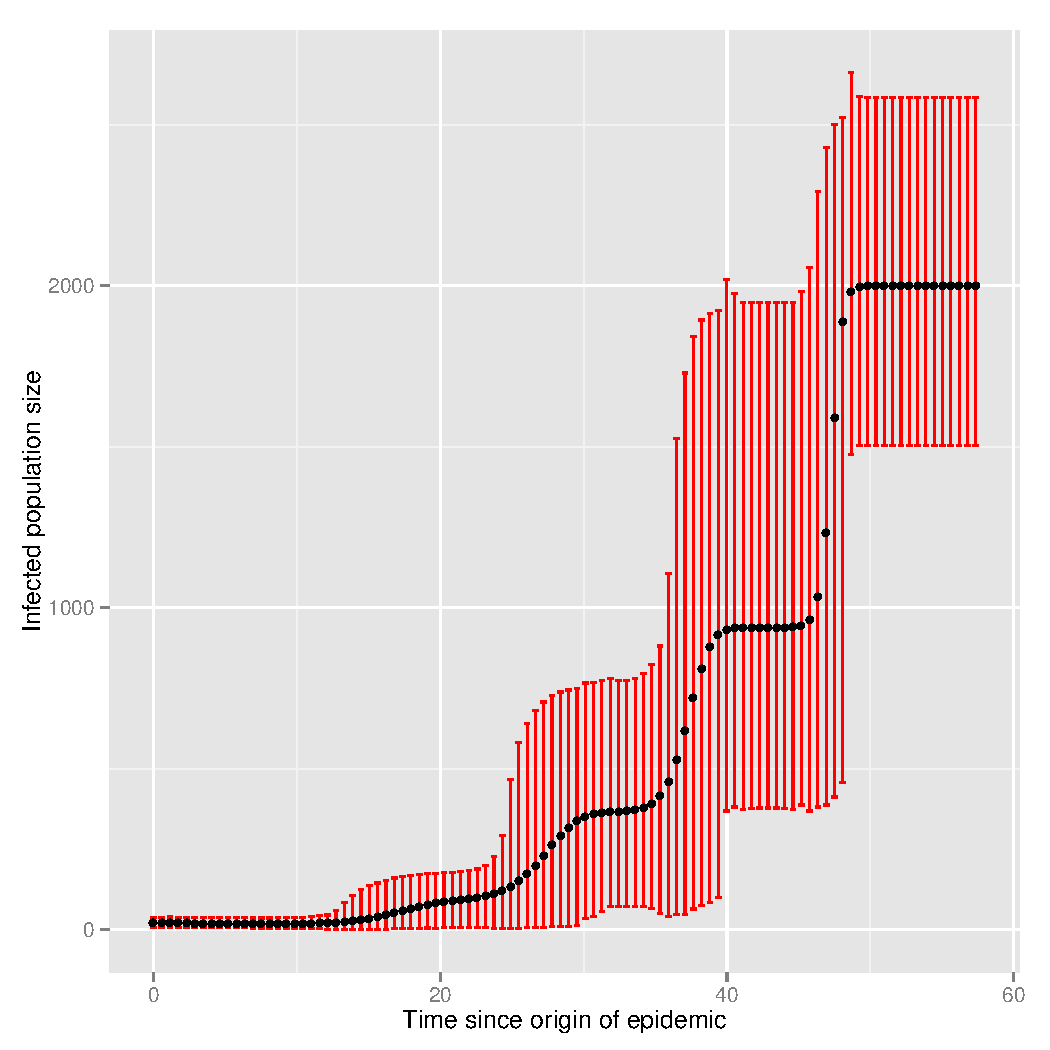
\includegraphics[width=3in]{popSize}
\caption{\footnotesize {\bf The means and 95 \% HPD intervals for posterior estimates of the infected population size through time.} 
The graph shows how the infected population size  grows through time for scG sample 1 epidemic 3 (the most recent sample from epidemic~3).} 
\label{fig: popSize} 
\end{figure}
\end{center} 

We cannot yet present the results from the analysis with birth-death skyline model with sampled ancestors as the analyses are incomplete. We anticipate to reporting estimates for parameters in a fixed number of intervals over the period of the epidemic: 
\vskip2mm

\begin{tabular} {cp{0.9\textwidth}}
$\delta$ & the total rate of removal due to death or sampling. $\delta$ is defined as  $\mu + \psi r$; \\

$R_e$ & the effective reproductive number defined as $\frac \lambda \delta$;  \\

$s$ & the sampling proportion, $\frac \psi {\mu + \psi}$; and\\

$r$ & the probability of removal at sampling; 
\end{tabular}

\vskip2mm

\noindent given that we know one of the parameters, $\mu$ for example.  

\section{Interpretation}

We can estimate the past epidemiological dynamics and estimate how the parameters driving the epidemic change over time.  Most properties of the epidemic that are not explicit parameters of the model (for example, the total number of infected) can be inferred either through analytic calculations based on estimated parameters, or further simulations.  

\section{Outlook}

 The computation time required for making reliable estimates is  long but feasible for datasets with approximately 300 samples. 


To use the birth-death model, we need information about one of the parameters such as the total removal rate, that is, the expected time from infection until the person stops causing other infectious due to treatment, behaviour change, or death.  Clinical observations such as known death times or observed behavioural changes from which informative priors could be drawn would help.




\section{Supplement}

Our model allows to estimate samples that are direct ancestors of other samples in a transmission chain and removal (from epidemic) at sampling probability. Figure~\ref{fig: SA} shows preliminary posterior estimates of sampled ancestors for one of the samples.  The mean estimate and 95\% HPD for $r$ was 0.9 [0.77, 0.98] for scA sample 1 epidemic 1. 

\begin{center} 
\begin{figure}[!h]
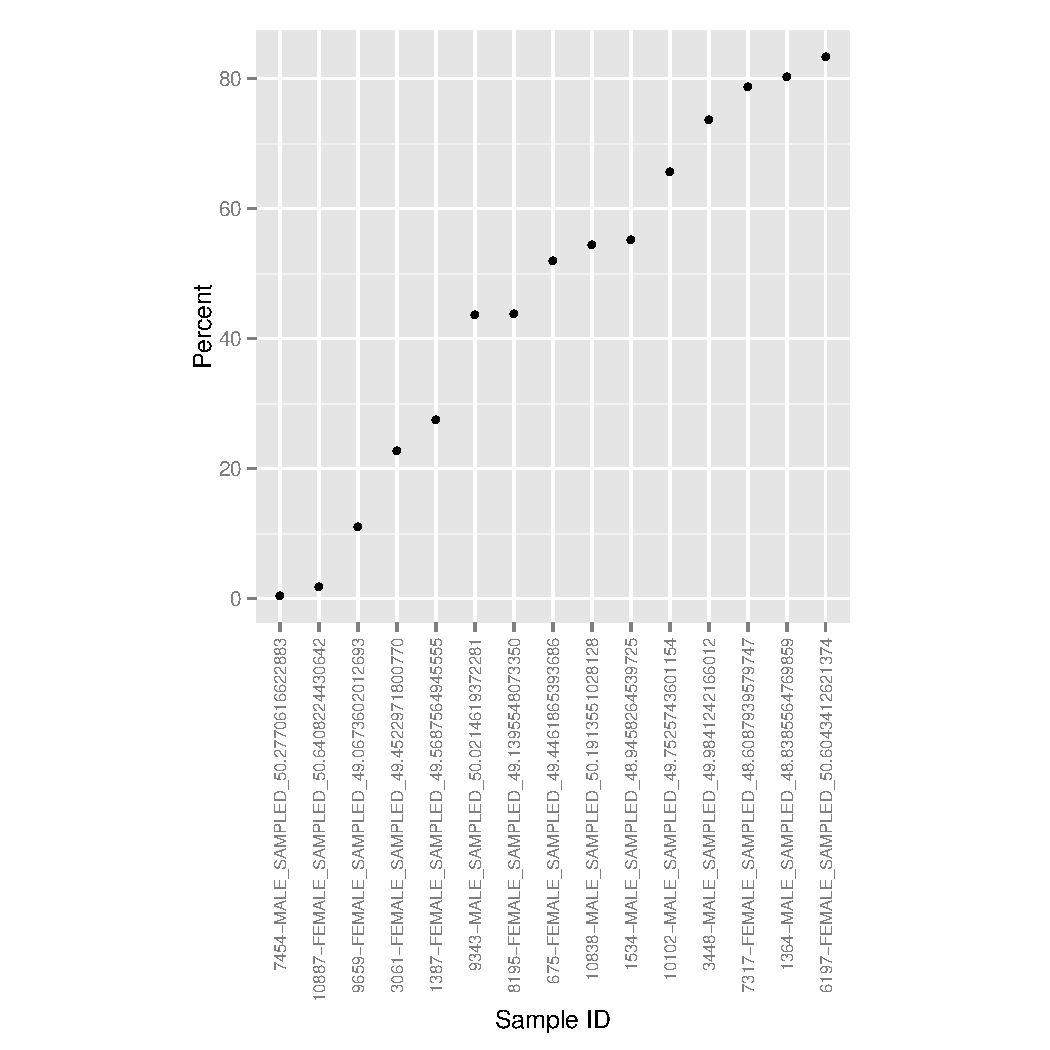
\includegraphics[width=4in]{sa_graph_scA}
\caption{\footnotesize {\bf Posterior probabilities of samples to be sampled ancestors.} 
The graph shows the posterior probabilities of samples to be sampled ancestors for scA sample 1 epidemic 1 (the most recent sample from epidemic 1). Only samples with non-zero probabilities are shown} 
\label{fig: SA} 
\end{figure}
\end{center} 

\end{document}
